\begin{figure}
  \centering
  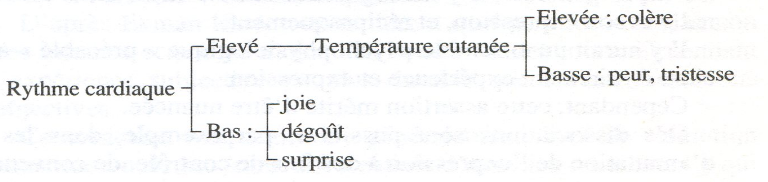
\includegraphics[width=10cm]{./Chapitre1/figures/Ekman1983.png}
  \caption{Traduction de la figure extraite de l'article de Paul Ekman et al.~\cite{Ekman1983} décrivant un arbre de décision pour déterminer l'émotion. On voit que la colère peut être détectée par un rythme cardiaque élevé et une température cutanée élevée.}
  \label{fig:Ekman1983}
\end{figure}
